\section{Impulse limit and free nuclear recoil}\label{sec:11.4}

A dark-matter particle of \SI{20}{MeV} can transfer up to $2\mchi v_{\mathrm{max}} = \SI{106}{keV}$ to a silicon nucleus. At $q = \SI{100}{keV}$ the free recoil energy is $E_R = \SI{191}{meV}$, three times the highest phonon energy, and the Poisson series of \cref{sec:11.3} has a mean of $2W_\kappa = 6.3$ phonons. Their sum is no longer a set of phonon bands. It is a single peak centered at $E_R$, \SI{88}{meV} wide, and as $q$ grows it narrows toward the delta function $\delta(\omega - E_R)$ of the free recoil that \cref{sec:1.3,sec:2.2} assumed. The nucleus recoils almost as if it were free, and what is left of the crystal is the motion of the nucleus in its well at the moment of the kick, which Doppler-broadens the line by an amount set by the kinetic energy of the nuclei; the standard nuclear-recoil rate with the Helm form factor is its limit, reached in silicon above 90 to \SI{140}{keV} depending on the criterion.

\subsection{The impulse approximation}

At $q = \SI{100}{keV}$, 44 times the zone momentum, the distinct part of the response is negligible (\cref{sec:11.3}), and each nucleus responds on its own. Its self correlation has an exact form that needs no phonons. The kick $\ee^{\ii\vect{q}\cdot\vect{X}}$ shifts the momentum of the nucleus by $\vect{q}$, and since every interaction in the crystal depends on the positions of the nuclei and not on their momenta, the kick changes only the kinetic energy $\vect{p}^2/2M_\kappa$. The Hamiltonian seen after the kick is the old one plus
\begin{equation*}
  D = E_R + \frac{\vect{q}\cdot\vect{p}}{M_\kappa} ,
\end{equation*}
the energy that the same kick would give a free particle of momentum $\vect{p}$. Its mean and variance follow exactly (\cref{app:D.32}). The mean energy deposited is $\langle D\rangle = E_R$, the sum rule \cref{eq:5.6-sum}. The variance is $\langle D^2\rangle - E_R^2 = q^2\langle p_{\hat q}^2\rangle/M_\kappa^2$, with $p_{\hat q} = \hat{\vect{q}}\cdot\vect{p}$, at any temperature and for any potential, anharmonic ones included. Defining the kinetic energy of the nucleus along the direction of the kick, $E^{\mathrm{kin}}_\kappa(\hat{\vect{q}}) = \langle p_{\hat q}^2\rangle/2M_\kappa$, the width of the response is
\begin{equation}
  \sigma_\omega = \bigl[4E_R\,E^{\mathrm{kin}}_\kappa(\hat{\vect{q}})\bigr]^{1/2} .
  \label{eq:11.4-width}
\end{equation}

If the nucleus were free, $D$ would commute with the Hamiltonian, and each momentum $\vect{p}$ would absorb exactly the energy $D$. For a bound nucleus the commutator is the force of the neighbors, and the \emph{impulse approximation} drops it: the nucleus is treated as free for the duration of the kick, with the momentum distribution $\mathfrak{f}_\kappa(\vect{p})$ that it has in the crystal, normalized to one.
\begin{keyresult}[Impulse approximation of the nuclear response]
\begin{equation}
  S_A(\vect{q},\omega) \simeq \frac{2\pi}{\Omega}\sum_\kappa c_\kappa^2\int\dd^3p\;\mathfrak{f}_\kappa(\vect{p})\;\delta\Bigl(\omega - \frac{q^2}{2M_\kappa} - \frac{\vect{q}\cdot\vect{p}}{M_\kappa}\Bigr) .
  \label{eq:11.4-IA}
\end{equation}
It keeps the exact mean $E_R$ and the exact width \cref{eq:11.4-width}. Its leading error is the third cumulant, at $T = 0$ equal to $c_3 = (q^2/2M_\kappa^2)\langle\partial_{\hat q}^2V\rangle$ with $V$ the Born--Oppenheimer surface, whose share of the shape falls as $1/q$ (\cref{app:D.32}).
\end{keyresult}
\noindent The term $\vect{q}\cdot\vect{p}/M_\kappa$ is a Doppler shift: a nucleus moving toward the kick absorbs more energy, one moving away absorbs less. The same picture underlies the impulse approximation of the electrons in \cref{we:4-gas}, where the Fermi momentum takes the place of the zero-point momentum, and neutron Compton scattering, which uses it to measure the momentum distributions of light nuclei in solids and liquids~\cite{andreani2005measurement}. The approximation is good when the kick is short compared with a vibration period. The time integral of the response is cut off at $t \sim 1/\sigma_\omega$, and the force of the neighbors changes the momentum during that time by a fraction $\sim\langle\omega\rangle/\sigma_\omega$ of its spread. At $T = 0$ this fraction is $x_R^{-1/2}$, with the recoil parameter $x_R = E_R/\langle\omega\rangle$ of \cref{sec:8.5}.

In a harmonic crystal $\mathfrak{f}_\kappa$ is a Gaussian at any temperature, since the momentum of each mode is Gaussian in a thermal state of an oscillator. Its width follows from the displacement correlation \cref{eq:5.6-C}. On a site of cubic symmetry, with the projected density of states $g_{\mathrm{ph},\kappa}/3$ of \cref{sec:11.3},
\begin{equation*}
  E^{\mathrm{kin}}_\kappa = \frac14\int\dd\omega\;\frac{g_{\mathrm{ph},\kappa}(\omega)}{3}\;\omega\coth\frac{\omega}{2T} ,
\end{equation*}
which at $T = 0$ is $\langle\omega\rangle/4$. Half the zero-point energy of each mode is kinetic, so a nucleus carries the kinetic energy $3\langle\omega\rangle/4$, a third of it along each direction. The impulse response of one species is then the Gaussian
\begin{equation}
  S_A(\vect{q},\omega) \simeq \frac{2\pi c_\kappa^2}{\Omega}\,\frac{1}{(2\pi\sigma_\omega^2)^{1/2}}\exp\Bigl[-\frac{(\omega - E_R)^2}{2\sigma_\omega^2}\Bigr] , \qquad
  \sigma_\omega^2 = E_R\,\Bigl\langle\omega\coth\frac{\omega}{2T}\Bigr\rangle ,
  \label{eq:11.4-IAgauss}
\end{equation}
which at $T = 0$ has $\sigma_\omega/E_R = x_R^{-1/2}$, the relative width that \cref{sec:8.5} found from the cumulants of the Poisson series. Campbell-Deem, Knapen, Lin and Villarama obtain it as the saddle point of the time integral at $t = 0$~\cite[Eqs.~(37)--(39)]{campbelldeem2022dark}. For a nucleus in an isotropic oscillator of frequency $\omega_0$, the spread $q(\omega_0/2M_\kappa)^{1/2}$ of Kahn, Krnjaic and Mandava~\cite[Eq.~(4)]{kahn2021dark} is the same width with $\langle\omega\rangle = \omega_0$. The harmonic crystal gives every cumulant (\cref{app:D.32}): $c_k = E_R\langle\omega^{k-1}\rangle$ for odd $k$, at any temperature, and $c_k = E_R\langle\omega^{k-1}\coth(\omega/2T)\rangle$ for even $k$. The skewness, $c_3/\sigma_\omega^3 = (\langle\omega^2\rangle/\langle\omega\rangle^2)\,x_R^{-1/2}$ at $T = 0$, is the leading correction to \cref{eq:11.4-IAgauss}. It moves the maximum of the spectrum below $E_R$ by about half the skewness times $\sigma_\omega$, while the mean stays at $E_R$.

In silicon the density of states of \cref{sec:5.2} gives $\langle\omega\rangle = \SI{40.9}{meV}$, so $E^{\mathrm{kin}}_\kappa = \SI{10.2}{meV}$ at $T = 0$, and $\langle\omega^2\rangle/\langle\omega\rangle^2 = 1.19$. The zero-point motion broadens the line as much as a classical gas at \SI{237}{K} would, the temperature at which $T/2$ equals $E^{\mathrm{kin}}_\kappa$. Heating the crystal changes this little until the thermal energy reaches the phonon energies: $E^{\mathrm{kin}}_\kappa$ rises by \SI{2}{\percent} at \SI{77}{K} and by \SI{56}{\percent} at \SI{300}{K}, where the width is 1.25 times its zero-temperature value. At the \SI{10}{mK} of a detector the zero-temperature values hold.

\Cref{fig:11-impulse} follows the silicon response from the multiphonon regime into the impulse regime. At $q = \SI{50}{keV}$, $x_R = 1.2$, the spectrum still shows the phonon bands: its maximum lies at $0.36\,E_R = \SI{17}{meV}$, on the transverse-acoustic peak of the single-phonon distribution, and a fifth of the weight is in the zero-phonon line. At \SI{100}{keV} the bands have merged into a peak whose maximum lies at $0.81\,E_R$. The Gaussian \cref{eq:11.4-IAgauss} has the right height and width there, and it misses by up to a fifth of the peak height, from the skewness and from the remaining structure of the phonon orders. At 200 and \SI{400}{keV} the deviations fall to 7 and \SI{3}{\percent} of the peak, roughly as $x_R^{-1/2}$, and the maximum approaches $E_R$.

\begin{figure}[tbp]
  \centering
  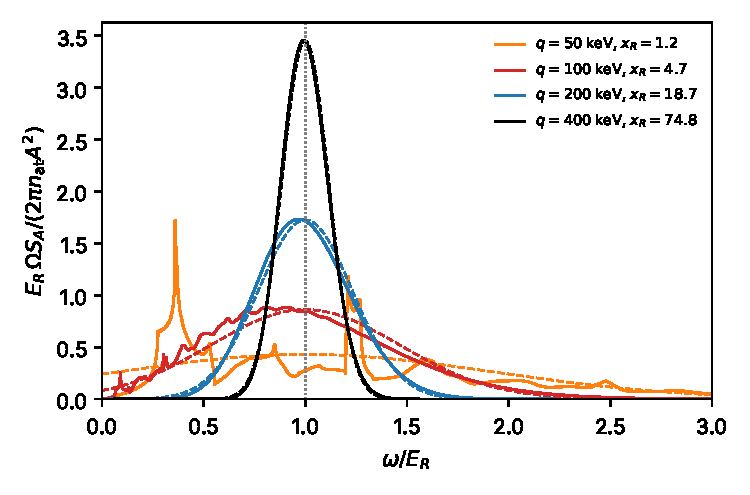
\includegraphics[width=\linewidth]{figures/ch11/fig11_4.pdf}
  \caption{Nuclear response of silicon at $T = 0$ per nucleus, $\Omega S_A/(2\pi n_{\mathrm{at}}A^2)$, times $E_R$, against $\omega/E_R$, at $q = 50$, 100, 200 and \SI{400}{keV} ($x_R = 1.2$, 4.7, 18.7 and 74.8). Solid: the incoherent response of \cref{eq:11.3-inc} summed over all phonon orders, from the density of states of the PBE force constants of \cref{sec:5.2}. It is evaluated by Fourier transform of the generating formula \cref{eq:5.6-gen}. The zero-phonon line, of weight $\ee^{-2W_\kappa} = 0.21$ at \SI{50}{keV} and below $2\times10^{-3}$ at the larger $q$, is not shown. Dashed: the impulse Gaussian \cref{eq:11.4-IAgauss}, mean $E_R$ and relative width $x_R^{-1/2}$. Dotted: the free recoil, $\omega = E_R$. The maximum of the spectrum lies at 0.36, 0.81, 0.97 and $0.99\,E_R$.}
  \label{fig:11-impulse}
\end{figure}

The width needs one number per species, the kinetic energy of the nucleus along $\hat{\vect{q}}$. The harmonic value comes from the same phonon calculation as the Debye--Waller exponent (\cref{sec:5.4,app:E.4}), as the first moment of the projected density of states instead of the inverse moment. Beyond the harmonic approximation the nuclear momentum distribution, its kinetic energy and the curvature that sets $c_3$ are computed by path-integral molecular dynamics, which treats the nuclei as quantum particles on the full Born--Oppenheimer surface; \cref{app:E.17} specifies that calculation for silicon, germanium and GaAs. The anharmonic change of $E^{\mathrm{kin}}_\kappa$ is the subject of \cref{sec:11.5}.

\begin{workedexample}{The impulse width at \SI{100}{keV} in silicon}\label{we:11-width}
Take a silicon nucleus, $M = \SI{26.162}{GeV}$, at $T = 0$ and $q = \SI{100}{keV}$. The free recoil energy is $E_R = q^2/2M = \SI{191.1}{meV}$, and with $\langle\omega\rangle = \SI{40.9}{meV}$ the recoil parameter is $x_R = 4.67$. The kinetic energy along $\hat{\vect{q}}$ is $\langle\omega\rangle/4 = \SI{10.23}{meV}$, and \cref{eq:11.4-width} gives
\begin{equation*}
  \sigma_\omega = (4 \times \SI{191.1}{meV} \times \SI{10.23}{meV})^{1/2} = \SI{88.4}{meV} , \qquad \frac{\sigma_\omega}{E_R} = 0.463 = x_R^{-1/2} .
\end{equation*}
The Doppler reading gives the same number. The nucleus moves along $\hat{\vect{q}}$ with the root-mean-square speed $(2E^{\mathrm{kin}}_\kappa/M)^{1/2} = \SI{265}{m.s^{-1}}$, while the kick gives it $q/M = \SI{1.15}{km.s^{-1}}$. The relative spread of $D$ is twice the ratio of the two speeds, 0.463.

The Gaussian has a full width at half maximum of \SI{208}{meV}, larger than $E_R$ itself. The full response of \cref{fig:11-impulse} at this $q$ has a width at half maximum of \SI{207}{meV}. The shape is skewed. The skewness is $1.19 \times 4.67^{-1/2} = 0.55$, which places the maximum about $0.55\,\sigma_\omega/2 = \SI{24}{meV}$ below $E_R$; the full response peaks at \SI{154}{meV}, \SI{37}{meV} below, because the phonon orders still leave ripples on the peak. At \SI{300}{K} the width grows to \SI{110}{meV}.

A germanium nucleus is 2.6 times heavier and its phonons are softer. With $\langle\omega\rangle \approx \SI{23.6}{meV}$, an estimate from its Debye temperature of \SI{373}{K} (below), the same $q$ gives $E_R = \SI{73.9}{meV}$, $x_R = 3.1$ and $\sigma_\omega/E_R = 0.57$: at equal momentum transfer the germanium response is further from free recoil than the silicon one.
\end{workedexample}

On the truncation label of \cref{sec:8.5}, \cref{eq:11.4-IA} is $\mathcal{K}$ = impulse with $n_B = 0$. It holds at any anharmonic order $n_A$ when $\mathfrak{f}_\kappa$ is the true momentum distribution, and the Gaussian \cref{eq:11.4-IAgauss} is its value at $n_A = 0$. Temperature enters only through $E^{\mathrm{kin}}_\kappa$, with all orders $n_T$ kept by the factor $\coth(\omega/2T)$.

\subsection{Free recoil and the standard rate}

As $x_R$ grows, the relative width $x_R^{-1/2}$ goes to zero and the Gaussian becomes $\delta(\omega - E_R)$~\cite[Eq.~(42)]{campbelldeem2022dark}. For a coupling to nucleons the vertex of a nucleus is $A_\kappa F_N(q)$, with the elastic form factor $F_N$ of \cref{eq:2.2-FN}. The nucleons move with their nucleus, and the momenta of the impulse regime, up to a few MeV for sub-GeV dark matter, are far too small to excite it internally. For one species the response is then $S_A = 2\pi\nd_NA^2F_N(q)^2\delta(\omega - q^2/2M)$, with $\nd_N = n_{\mathrm{at}}/\Omega$ the number density of nuclei. Insert it into \cref{eq:8.2-spectrum} with one row, $\mathfrak{D} = |\tilde V_N|^2$. The response does not depend on $\hat{\vect{q}}$, so the angle between $\vect{q}$ and $\vect{v}$ can be integrated first: $\int\dd^3q/(2\pi)^3$ of $\delta(\omega - \vect{q}\cdot\vect{v} + q^2/2\mchi)$ gives $\int q\,\dd q\,\Theta(v - \vmin)/(4\pi^2v)$, as in \cref{sec:1.3}, and the average over $f_\chi$ turns $\Theta/v$ into $\eta(\vmin)$ of \cref{eq:1.3-eta}. With $\rho_T = \nd_NM$,
\begin{equation*}
  \frac{\dd\mathcal{R}}{\dd\omega} = \frac{\rho_\chi}{\mchi\,\nd_NM}\int\frac{q\,\dd q}{4\pi^2}\,|\tilde V_N|^2\,2\pi\nd_NA^2F_N^2\,\delta\Bigl(\omega - \frac{q^2}{2M}\Bigr)\,\eta(\vmin)
  = \frac{\rho_\chi A^2|\tilde V_N|^2}{2\pi\mchi}\,F_N(q)^2\,\eta(\vmin) ,
\end{equation*}
at $q = (2M\omega)^{1/2}$, and \cref{eq:1.3-vmin} with $\Delta_\chi = 0$ gives $\vmin = q/2M + q/2\mchi = q/2\mu_{\chi N}$. A heavy mediator, $|\tilde V_N|^2 = \pi\sigma_p/\mu_{\chi p}^2$, with $\sigma_N = \sigma_pA^2\mu_{\chi N}^2/\mu_{\chi p}^2$ from \cref{eq:2.2-nucleus}, gives
\begin{keyresult}[Free nuclear recoil as the impulse limit]
\begin{equation}
  \frac{\dd\mathcal{R}}{\dd E_R} = \frac{\rho_\chi\,\sigma_N}{2\mchi\,\mu_{\chi N}^2}\,F_N(q)^2\,\eta(\vmin) , \qquad q = (2ME_R)^{1/2} , \qquad \vmin = \frac{q}{2\mu_{\chi N}} ,
  \label{eq:11.4-LS}
\end{equation}
the spin-independent recoil spectrum of \cref{sec:2.2}, with $\sigma_N$ of \cref{eq:2.2-nucleus}. It is the limit $x_R \to \infty$ of the crystal response.
\end{keyresult}
\noindent This is the standard rate of nuclear-recoil searches~\cites{lewin1996review}[Eq.~(104)]{lin2019tasi}, and with $F_N$ the Helm form \cref{eq:2.2-helm} and the Lewin--Smith parameters of \cref{sec:2.2} it is the rate that experiments quote. Kahn and Lin reach the same spectrum from an Einstein oscillator, whose Poisson distribution of phonon numbers concentrates at $E_R/\omega_0$ for large $q$~\cite[Sect.~IV\,A, Eqs.~(90)--(92)]{kahn2022searches}. On the truncation label the free recoil is $\mathcal{K}$ = impulse at zero width, $n_B = 0$; its mean deposit is exact at every anharmonic order and temperature, and only the width depends on them.

The derivation says what the formula needs: a recoil parameter large enough that the response is a narrow peak, and a rate whose weight in $\omega$, the factor $\eta(\vmin)$ together with the threshold, does not vary across the width $\sigma_\omega$. \Cref{lim:11.4a} tests both in silicon, by computing the heavy-mediator rate from the full multiphonon response and dividing it by \cref{eq:11.4-LS}. For a particle of \SI{1}{GeV}, whose kinematic endpoint lies far above the energies shown, the two agree within \SI{10}{\percent} for $x_R \ge 2.3$, or $E_R \ge \SI{93}{meV}$ and $q \ge \SI{70}{keV}$, and within \SI{2}{\percent} for $x_R \ge 4.3$. The free form works where the spectrum is not yet narrow, as Campbell-Deem and collaborators observed~\cite[Sect.~III\,D]{campbelldeem2022dark}, because a smooth weight averages over the peak and the mean of the peak is exactly $E_R$. Below $x_R \approx 2$ the deposit comes in whole phonons, and the ratio swings by factors of two with the bands of the phonon spectrum.

A lighter particle has its endpoint $2\mu_{\chi N}^2v_{\mathrm{max}}^2/M$ close to the energies that matter, and there $\eta$ falls steeply across the peak. For \SI{50}{MeV} the endpoint is at \SI{1.34}{eV}, $x_R = 32.7$. Between $x_R = 3$ and 8 the free form overestimates the crystal rate by 5 to \SI{21}{\percent}, because the width spreads each momentum transfer over a range of energies across which $\eta$ falls steeply. From $x_R = 14$ upward, however, $4.9\,\sigma_\omega$ below the endpoint, the crystal rate exceeds the free one by more than \SI{10}{\percent} and keeps rising. Above the endpoint the free recoil gives nothing, while the Doppler tail of the bound nucleus still deposits energy. This is the impulse-regime counterpart of the Poisson tail of \cref{we:11-tail}, and the reason Kahn, Krnjaic and Mandava found that a bound nucleus extends the reach of a detector below the masses that elastic kinematics allows~\cite[text after Eq.~(4)]{kahn2021dark}. The impulse Gaussian \cref{eq:11.4-IAgauss}, used in the same rate integral, follows the full crystal result within \SI{5}{\percent} from $x_R \approx 3.6$ at \SI{1}{GeV} and 3.8 at \SI{50}{MeV}, up to three quarters of the endpoint, and it captures the endpoint tail too.

\begin{limitbox}[Free nuclear recoil with the Helm form factor][lim:11.4a]
For $x_R \gg 1$ the nuclear response becomes $(2\pi/\Omega)\sum_\kappa c_\kappa^2\delta(\omega - q^2/2M_\kappa)$~\cite[Eqs.~(39), (42)]{campbelldeem2022dark}, and the rate is the free recoil \cref{eq:11.4-LS} with $F_N = F_{\mathrm{Helm}}$ and the Lewin--Smith parameters~\cites{lewin1996review}[Eq.~(104)]{lin2019tasi}.
\par\smallskip
{\centering
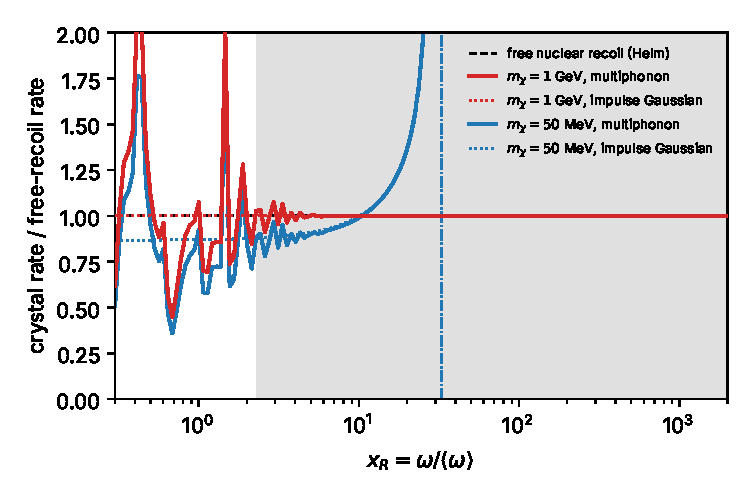
\includegraphics[width=\linewidth]{figures/ch11/limit11_4a.pdf}
\captionof{figure}{Heavy-mediator recoil rate of silicon per unit mass from the crystal response, divided by the free-recoil rate \cref{eq:11.4-LS} at $E_R = \omega$, against $x_R = \omega/\langle\omega\rangle$ with $\langle\omega\rangle = \SI{40.9}{meV}$. Solid: incoherent multiphonon response at $T = 0$, all orders, from the PBE density of states of \cref{sec:5.2}, integrated over $q$ with $\eta(\vmin)$ of the halo of \cref{sec:1.2} and the Helm form factor, for $\mchi = \SI{1}{GeV}$ (red) and \SI{50}{MeV} (blue). Dotted: the same with the impulse Gaussian \cref{eq:11.4-IAgauss}, the leading correction. Dash-dotted: the free-recoil endpoint at \SI{50}{MeV}. Gray band: $x_R \ge 2.3$, where the \SI{1}{GeV} rate stays within \SI{10}{\percent} of the free one. The lighter particle departs from it within about five widths $\sigma_\omega$ of its endpoint.}\label{fig:11-limit-4a}
\par}
\smallskip
Below $x_R \approx 2$ the energy arrives in whole phonons and the rate follows the phonon bands; near the kinematic endpoint the Doppler width of the bound nucleus feeds energies that a free nucleus cannot reach.
\end{limitbox}

Where does the impulse regime begin? The onset depends on the criterion. The relative width $x_R^{-1/2}$ falls to one half at $x_R = 4$, where the impulse Gaussian reproduces the rate of the limit check within \SI{5}{\percent}. This is $q = 2(2M\langle\omega\rangle)^{1/2}$, the boundary above which Campbell-Deem and collaborators replace the multiphonon sum by the Gaussian~\cite[text after Eq.~(39)]{campbelldeem2022dark}. In silicon it lies at $q = \SI{92.5}{keV}$, $E_R = \SI{164}{meV}$. The stricter criterion of \cref{sec:8.5}, a width below a third of $E_R$, needs $x_R \ge 9$, at \SI{139}{keV} and \SI{0.37}{eV}. For germanium a rough $\langle\omega\rangle$ is enough, and its Debye temperature of \SI{373}{K} supplies one (\cref{tab:5-phonons}): the Debye mean $\frac34\omega_{\mathrm{D}} = \SI{24.1}{meV}$, scaled by the ratio 0.981 of the computed to the Debye mean in silicon, gives $\langle\omega\rangle \approx \SI{23.6}{meV}$. The onsets are then $q = \SI{113}{keV}$ and $E_R = \SI{95}{meV}$ at $x_R = 4$, and \SI{170}{keV} and \SI{0.21}{eV} at $x_R = 9$. The heavier nucleus needs a larger momentum transfer but a smaller recoil energy. These onsets are not the \SI{93.4}{keV} of \cref{we:11-tail}, which is the momentum at which a free nucleus would first deposit three Debye energies. A particle much lighter than the nucleus reaches $q$ only if $2\mchi v_{\mathrm{max}} \ge q$, so the impulse regime is available in silicon from $\mchi = \SI{17.5}{MeV}$ and in germanium from \SI{21.3}{MeV} ($x_R = 4$), or from 26.2 and \SI{32.0}{MeV} ($x_R = 9$). Even then, as the limit check shows, the free form needs the energies of interest to lie several widths below the endpoint.

The impulse approximation leaves the crystal at the moment of the kick. It ignores the motion of the nucleus after the kick, and it leaves out anharmonicity, electronic excitation and the displacement of the atom. The kinetic energy and curvature of an anharmonic crystal shift $\sigma_\omega$ and $c_3$ (\cref{sec:11.5}), but never the mean. The electrons follow the nucleus at $n_B = 0$; the probability that the kick leaves them excited is the Migdal effect of \cref{chap:12}. With the electrons included, the third moment of the full nuclear response contains the electron density at the nucleus and is dominated by those excitations (\cref{sec:12.5}); the curvature in $c_3$ above is that of the Born--Oppenheimer surface alone. And a recoil above the displacement threshold of the lattice ejects the atom from its site, which changes how the energy is shared among phonons, defects and ionization (\cref{chap:19}) but not the response \cref{eq:11.4-IA}, since the momentum and energy are transferred before the atom moves.

\subsection{Fermionic absorption on nuclei}

A fermion $\chi$ of \SI{10}{MeV} that is absorbed on a silicon nucleus and leaves as a massless $\tilde\nu$ transfers the momentum $q = \mchi - \omega \simeq \SI{10}{MeV}$, and a free nucleus recoils with $E_R = \mchi^2/2M = \SI{1.91}{keV}$. Scattering at the same mass deposits at most $2\mu_{\chi N}^2v_{\mathrm{max}}^2/M = \SI{54}{meV}$. Absorption reaches recoil energies $1/4v_{\mathrm{max}}^2$ times larger, and because the momentum transfer is set by the rest energy, the deposit is a line, whatever the velocity distribution~\cite{dror2020direct}. \Cref{sec:10.9} built the rate for the operators $\Lambda_F^{-2}(\bar{\tilde\nu}P_L\chi)(\bar\psi\psi)$ and $\Lambda_F^{-2}(\bar{\tilde\nu}\gamma_\mu P_R\chi)(\bar\psi\gamma^\mu\psi)$, \cref{eq:10.9-ferm}. For nucleons in place of electrons only the response changes. The vector operator gives $(\sigma_F/2\pi)\bar S_{nn}(q,\omega)$, with $\sigma_F = \mchi^2/4\pi\Lambda_F^4$ and $\bar S_{nn}$ the direction-averaged response of the nucleon density, because continuity, exact for the nucleon current, turns the longitudinal current into the density and multiplies it by $(\mchi/q)^2$. With the dark matter at rest, $p = (\mchi, \vect{0})$, a massless outgoing fermion of four-momentum $(q, -\vect{q})$ and the nucleon current $J = (\rho, (\omega/q)\rho\,\hat{\vect{q}})$ fixed by continuity, the spin-summed contraction is $\mchi^3\rho^2/q$ for the vector operator and $\mchi q\rho^2$ for the scalar density; their ratio is $q^2/\mchi^2$. The transverse current of a nucleus is smaller by a factor of order $E^{\mathrm{kin}}_\kappa/M$ or $q^2/M^2$ and is dropped.

For a nucleus at rest, $\bar S_{nn} = 2\pi\nd_NA^2F_N(q)^2\delta(\omega - q^2/2M)$. Along the line $q = \mchi - \omega$ the argument of the delta function has the slope $1 + q/M$, and
\begin{keyresult}[Fermionic absorption on nuclei]
\begin{equation}
  \varGamma_V = \frac{\sigma_F\,\nd_NA^2F_N(q_{\mathrm{abs}})^2}{1 + q_{\mathrm{abs}}/M} = \sigma_F\,\nd_NA^2F_N^2\Bigl(1 - \frac{\mchi}{M} + \dots\Bigr) , \qquad \mchi = q_{\mathrm{abs}} + \frac{q_{\mathrm{abs}}^2}{2M} ,
  \label{eq:11.4-ferm-nuc}
\end{equation}
per dark-matter particle, in a target of free nuclei, at a recoil energy $E_R = q_{\mathrm{abs}}^2/2M \simeq \mchi^2/2M$; the event rate per unit mass is $(\rho_\chi/\mchi\rho_T)\varGamma_V$. In a crystal, in the incoherent approximation and for $\mchi$ not within a relative $v$ of the length of a reciprocal-lattice vector, the factor $1 - \ee^{-2W_\kappa(q_{\mathrm{abs}})}$ multiplies the rate.
\end{keyresult}
\noindent Since $\sigma_F \propto \mchi^2$, the rate carries the factor $\mchi^2(1 - \mchi/M)$. The scalar operator weights the density by $q^2/\mchi^2$ in addition and gives $\mchi^2(1 - 2\mchi/M)$. The difference is the longitudinal current: the density row alone has twice the recoil correction, and continuity halves it. Dror, Elor and McGehee write the rate per target nucleus as $(\rho_\chi/\mchi)\sigma_FA^2F_N^2$ for the vector operator, with the Helm form factor at $q = \mchi$~\cite[Eqs.~(1) and (4)]{dror2020direct}, which is \cref{eq:11.4-ferm-nuc} at $M \to \infty$. In silicon the recoil factor reaches \SI{10}{\percent} only at $\mchi = \SI{3}{GeV}$, where $q_{\mathrm{abs}}$ lies far beyond the first zero of the Helm form factor, at \SI{256}{MeV}, and elastic absorption is negligible; on a proton target it is about \SI{10}{\percent} at \SI{100}{MeV}.

The crystal changes the rate at the other end of the mass range. In the response of \cref{sec:11.3} the zero-phonon term conserves crystal momentum and deposits no energy, so it absorbs a fermion only if $|\vect{q}| = \mchi$ equals the length of a reciprocal-lattice vector, to within the relative spread $v$ of the dark-matter momenta. At any other mass the lattice must take up the momentum with at least one phonon, and in the incoherent approximation the weight of those terms is $1 - \ee^{-2W_\kappa}$, evaluated at $q = q_{\mathrm{abs}}$. Along the line $q = \mchi - \omega$ the momentum changes by $\omega$, a fraction $E_R/\mchi = \mchi/2M$ of itself, which rebuilds the factor $1/(1 + q_{\mathrm{abs}}/M)$ in the impulse regime and is negligible below it. In silicon, with $2W_\kappa = q^2\langle u_x^2\rangle$, this is 0.061 at $\mchi = \SI{10}{keV}$, 0.43 at \SI{30}{keV} and 0.90 at \SI{60.5}{keV}. The free-nucleus formula therefore overestimates the absorption rate by a factor of 16 at \SI{10}{keV}, and it holds to \SI{10}{\percent} only above \SI{61}{keV}, the boundary of \cref{lim:11.4b}. Below about \SI{100}{keV} the deposit is not a line at $\mchi^2/2M$ either. It is the multiphonon spectrum of \cref{sec:11.3} at $q = \mchi$: mostly one phonon below about \SI{20}{keV}, a few phonons up to the impulse onset near \SI{90}{keV}, and the Gaussian \cref{eq:11.4-IAgauss} above it. The weights of the lowest orders carry the coherence corrections of \cref{sec:11.3}, below \SI{10}{\percent} above about \SI{6.6}{keV} for two and three phonons and above \SI{18}{keV} for one.

Above the onset the crystal sets the width of the line. The impulse Gaussian has the relative width $x_R^{-1/2} = (2M\langle\omega\rangle)^{1/2}/q_{\mathrm{abs}} = \SI{46.3}{keV}/\mchi$ in silicon: \SI{4.6}{\percent} at \SI{1}{MeV}, \SI{0.46}{\percent} at \SI{10}{MeV}. The motion of the dark matter shifts the recoil energy by $-2v\cos\theta$ in relative terms, with $\theta$ the angle between its velocity and the outgoing $\tilde\nu$. For the halo of \cref{sec:1.2}, whose root-mean-square speed in the laboratory is \SI{379}{km.s^{-1}}, the root-mean-square shift is $2(\langle v^2\rangle/3)^{1/2} = 1.5\times10^{-3}$, the relative width $\sim10^{-3}$ that Dror, Elor and McGehee attribute to corrections to the leading kinematics~\cite{dror2020direct}. The two widths are equal at $\mchi = \SI{32}{MeV}$, and below that mass the line in a crystal is broader than the halo makes it, by the zero-point motion of the nuclei.

\begin{limitbox}[Fermionic absorption on nuclei][lim:11.4b]
A fermion absorbed on free nuclei gives the rate $(\rho_\chi/\mchi)\sigma_FA^2F_N^2$ per nucleus, with $\sigma_F = \mchi^2/4\pi\Lambda_F^4$, at the recoil energy $\mchi^2/2M$~\cite[Eqs.~(1), (3) and (4)]{dror2020direct}.
\par\smallskip
{\centering
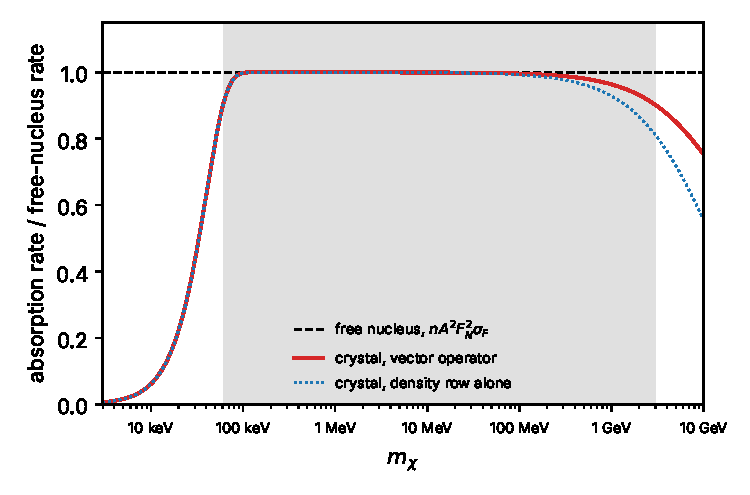
\includegraphics[width=\linewidth]{figures/ch11/limit11_4b.pdf}
\captionof{figure}{Absorption rate of a fermion on silicon nuclei, divided by the free-nucleus rate of the limit check, against $\mchi$, with the nuclear form factor divided out of both. Solid: the vector operator in the crystal, $[1 - \ee^{-2W_\kappa(q_{\mathrm{abs}})}]/(1 + q_{\mathrm{abs}}/M)$ from \cref{eq:11.4-ferm-nuc}, incoherent approximation at $T = 0$ with $\langle u_x^2\rangle = \SI{2.45e-3}{\angstrom^2}$ from the PBE density of states of \cref{sec:5.2}. Dotted: the density row alone, as for the scalar operator, with the recoil factor $(1 - \mchi/M)^2$ to leading order instead of $1 - \mchi/M$. Gray band: $\SI{61}{keV} \le \mchi \le \SI{3.0}{GeV}$, where the vector rate is within \SI{10}{\percent} of the free one.}\label{fig:11-limit-4b}
\par}
\smallskip
Below about \SI{60}{keV} in silicon the absorption must create phonons and the free-nucleus rate overcounts it by $\ee^{-2W_\kappa}/(1 - \ee^{-2W_\kappa})$; above a few GeV the recoil factor $1 - \mchi/M$ and the form factor at $q_{\mathrm{abs}}$ instead of $\mchi$ matter.
\end{limitbox}

\noindent On the truncation label the limit check sits at $n_B = 0$ and $n_T = 0$, with $\mathcal{K}$ = multiphonon (incoherent, all orders) below the impulse onset and $\mathcal{K}$ = impulse above it.
